\documentclass{beamer}
\usepackage[utf8]{inputenc}
\usetheme{Madrid}
\usecolortheme{default}
\usepackage{amsmath,amssymb,amsfonts,amsthm}
\usepackage{txfonts}
\usepackage{tkz-euclide}
\usepackage{listings}
\usepackage{adjustbox}
\usepackage{array}
\usepackage{tabularx}
\usepackage{gvv}
\usepackage{lmodern}
\usepackage{circuitikz}
\usepackage{tikz}
\usepackage{graphicx}

\setbeamertemplate{page number in head/foot}[totalframenumber]

\usepackage{tcolorbox}
\tcbuselibrary{minted,breakable,xparse,skins}

\definecolor{bg}{gray}{0.95}
\DeclareTCBListing{mintedbox}{O{}m!O{}}{%
  breakable=true,
  listing engine=minted,
  listing only,
  minted language=#2,
  minted style=default,
  minted options={%
    linenos,
    gobble=0,
    breaklines=true,
    breakafter=,,
    fontsize=\small,
    numbersep=8pt,
    #1},
  boxsep=0pt,
  left skip=0pt,
  right skip=0pt,
  left=25pt,
  right=0pt,
  top=3pt,
  bottom=3pt,
  arc=5pt,
  leftrule=0pt,
  rightrule=0pt,
  bottomrule=2pt,
  toprule=2pt,
  colback=bg,
  colframe=orange!70,
  enhanced,
  overlay={%
    \begin{tcbclipinterior}
    \fill[orange!20!white] (frame.south west) rectangle ([xshift=20pt]frame.north west);
    \end{tcbclipinterior}},
  #3,
}
\lstset{
    language=C,
    basicstyle=\ttfamily\small,
    keywordstyle=\color{blue},
    stringstyle=\color{orange},
    commentstyle=\color{green!60!black},
    numbers=left,
    numberstyle=\tiny\color{gray},
    breaklines=true,
    showstringspaces=false,
}

\title{Matgeo-q.3.4.5}
\author{AI25BTECH11036-SNEHAMRUDULA}
\date{\today} 

\begin{document}

\begin{frame}
\titlepage
\end{frame}

\section*{Outline}
\begin{frame}{question}
    \textbf{3.4.5} Construct a rhombus whose side is of length $3.4 \, \text{cm}$ and one of its angles is $45^\circ$.
\end{frame}

\begin{frame}[allowframebreaks]{solution}
Let the side length be 
\begin{align}
    s &= 3.4                                            \label{eq:rhomb1}
\end{align}
and the given angle be
\begin{align}
    \theta &= 45^\circ.                                 \label{eq:rhomb2}
\end{align}

\noindent
We now place the vertices of the rhombus as follows:
\begin{align}
    \vec{A} &= \myvec{0\\0},                            \label{eq:rhombA}\\
    \vec{B} &= s\myvec{1\\0},                           \label{eq:rhombB}\\
    \vec{D} &= s\myvec{\cos\theta\\ \sin\theta}.        \label{eq:rhombD}
\end{align}

\framebreak % ---- forces continuation on next slide ----

\noindent
The fourth vertex is obtained using the parallelogram law:
\begin{align}
    \vec{C} &= \vec{B} + \vec{D} - \vec{A}.             \label{eq:rhombC}
\end{align}
\noindent
Thus, the coordinates of the rhombus are
\begin{align}
    \vec{A} &= \myvec{0\\0},                            \label{eq:rhombA2}\\
    \vec{B} &= \myvec{3.4\\0},                          \label{eq:rhombB2}\\
    \vec{D} &= \myvec{\tfrac{3.4}{\sqrt{2}}\\ \tfrac{3.4}{\sqrt{2}}}, 
                                                      \label{eq:rhombD2}\\
    \vec{C} &= \myvec{3.4+\tfrac{3.4}{\sqrt{2}}\\ \tfrac{3.4}{\sqrt{2}}}.
                                                      \label{eq:rhombC2}
\end{align}

\framebreak % ---- if needed, continue further ----

\noindent
Verification of equal sides:
\begin{align}
    \norm{\vec{B}-\vec{A}} &= s,                        \label{eq:check1}\\
    \norm{\vec{D}-\vec{A}} &= s,                        \label{eq:check2}\\
    \norm{\vec{C}-\vec{B}} &= s,                        \label{eq:check3}\\
    \norm{\vec{C}-\vec{D}} &= s.                        \label{eq:check4}
\end{align}

\noindent
Hence, $ABCD$ is a rhombus with side length $s=3.4$ cm and $\angle DAB = \theta = 45^\circ$.
\end{frame}

\begin{frame}{Graphical Representation}
   \begin{figure}[h!]
\centering
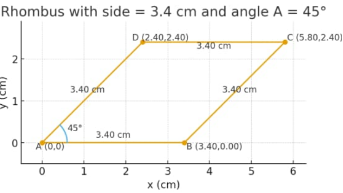
\includegraphics[width=0.6\linewidth]{fig3.4.5.png}
\end{figure}
\end{frame}

\end{document}